% ============================================================
%  SECTION 3: METHODOLOGY
% ============================================================
\section{Methodology}
\label{sec:methodology}

This section describes the complete experimental pipeline designed to address the three research
questions posed in this study. The pipeline comprises four tightly coupled stages: dataset
construction and preprocessing, model architecture definition, multi-phase training, and
systematic evaluation. All experiments are reproducible; dataset splits, random seeds, and
hyperparameters are fixed and reported below.

% ------------------------------------------------------------
\subsection{Dataset Construction and Preprocessing}
\label{sec:data}

A purpose-built corpus of 5{,}000 Amharic sentence pairs and task instances was assembled to
cover the linguistic phenomena most relevant to agentic conversational intelligence.  The corpus
spans four task types distributed as shown in Table~\ref{tab:dataset}: Translation (40\,\%),
Conversation (25\,\%), Morphology (20\,\%), and Ambiguity/Coreference (15\,\%).  This
distribution reflects the relative frequency of each phenomenon in real-world Amharic discourse
while ensuring sufficient minority-class coverage for statistical reliability.

\begin{table}[htbp]
  \centering
  \caption{Dataset Composition by Task Type}
  \label{tab:dataset}
  \begin{tabularx}{\columnwidth}{lrrX}
    \toprule
    \textbf{Task Type} & \textbf{Count} & \textbf{Proportion (\%)} & \textbf{Representative Phenomena} \\
    \midrule
    Translation                & 2{,}000 & 40.0 & Negated gerundive, temporal clauses, simple past \\
    Conversation               & 1{,}250 & 25.0 & Context, gratitude/resolution, tech inquiry \\
    Morphology                 & 1{,}000 & 20.0 & Causative, reciprocal/passive, near-future prefixes \\
    Ambiguity / Coreference    &   750 & 15.0 & Person ambiguity, suffix-based reference, conditionals \\
    \midrule
    \textbf{Total}             & \textbf{5{,}000} & \textbf{100.0} & -- \\
    \bottomrule
  \end{tabularx}
\end{table}

Each instance carries the fields \texttt{Amharic\_Text}, \texttt{English\_Text / Task\_Output},
and \texttt{Notes}, the last encoding fine-grained linguistic annotations (e.g.,
\emph{``Derived: Causative prefix; Base: Imperative masculine''}).

\subsubsection{Normalization Pipeline (\texttt{preprocess.py})}

Amharic orthography presents a well-documented homophone-homograph challenge: several
Ge\textquotesingle ez Fidel characters share identical phonology yet appear interchangeably in
written text~\cite{gasser2010,gezahen2015}.  A four-step normalization procedure was applied:

\begin{enumerate}
  \item \textbf{NFKC Unicode normalization.}  Compatibility characters are mapped to their
        canonical equivalents, removing invisible formatting differences introduced by different
        input methods.
  \item \textbf{Amharic-specific character mapping.}  Eleven character equivalence classes are
        collapsed to a canonical representative
        (e.g., \textipa{\textglotstop}/\textit{ሃ, ኃ, ሓ, ሐ} $\rightarrow$ \textit{ሀ};
        \textit{ፀ} $\rightarrow$ \textit{ጸ}).  This step directly addresses the
        script-awareness requirement of RQ2 at the preprocessing level.
  \item \textbf{Noise removal.}  Characters outside the Ge\textquotesingle ez block
        (U+1200--U+137F), standard ASCII alphanumerics, and Ethiopian punctuation
        (\textit{፦, ፣, ፤, ፥}) are replaced with a single space.
  \item \textbf{Whitespace normalization.}  Consecutive spaces are collapsed.
\end{enumerate}

The corpus was partitioned using stratified sampling (stratified by \texttt{Type}) with a fixed
random seed of 42 to ensure reproducibility: 70\,\% training (3{,}500 samples), 15\,\%
validation (750 samples), and 15\,\% test (750 samples).

% ------------------------------------------------------------
\subsection{Model Architectures}
\label{sec:models}

Three model architectures of increasing capability were implemented (\texttt{model\_defs.py}),
forming an ablation ladder that isolates the contribution of each innovation.

\subsubsection{Baseline Model}

The baseline is a standard encoder-only transformer built upon
\texttt{microsoft/Multilingual-MiniLM-L12-H384}~\cite{wang2020minilm}, a compact multilingual
model with 12 layers and a 384-dimensional hidden state.  A linear classification head is
attached to the \texttt{[CLS]} token representation:
%
\begin{equation}
  \hat{y} = W_c \, h_{\text{CLS}}, \quad W_c \in \mathbb{R}^{d_h \times C}
  \label{eq:baseline_cls}
\end{equation}
%
where $d_h = 384$ and $C$ is the number of output classes.  Subword tokenization via the
SentencePiece vocabulary shared across languages is used without modification.  This model
serves as the lower-bound reference that lacks both Ge\textquotesingle ez script awareness and
agentic reasoning.

\subsubsection{Script-Aware Model}

The \texttt{ScriptAwareModel} augments the baseline with a dedicated character-level branch
tailored to the Ge\textquotesingle ez alphabet.  Ge\textquotesingle ez (Fidel) comprises
approximately 500 distinct characters organized in syllabic orders; standard multilingual
tokenizers routinely merge these into coarse-grained subword units, losing phonological and
morphological distinctions encoded at the character level.

The character branch consists of:
\begin{itemize}
  \item \textbf{Character embedding matrix} $E_c \in \mathbb{R}^{500 \times 64}$ covering the
        complete Ge\textquotesingle ez character inventory.
  \item \textbf{1-D convolutional layer} with 128 output channels and kernel size 3,
        extracting local $n$-gram features from the character sequence of each token.
  \item \textbf{Adaptive average pooling} producing a fixed-length 128-dimensional character
        representation $h_c$ regardless of word length.
\end{itemize}

The character representation is concatenated with the subword hidden state and projected back to
the model dimension via a learned fusion layer:
%
\begin{equation}
  h_{\text{fused}} = \text{ReLU}\!\left(W_f \, [h_{\text{sub}}; h_c]\right),
  \quad W_f \in \mathbb{R}^{(d_h + 128) \times d_h}
  \label{eq:fusion}
\end{equation}
%
The fused \texttt{[CLS]} representation is then passed to the classification head.  This
architecture directly answers RQ2 by providing the model with high-fidelity, script-level
reading of Amharic input.

\subsubsection{Agentic Processor}

The \texttt{AgenticProcessor} treats inference as a multi-stage orchestration pipeline
(\texttt{model\_defs.py, AgenticProcessor.process}), decomposing the understanding of an
Amharic utterance into three explicitly reasoned sub-tasks before committing to a final
prediction:

\begin{enumerate}
  \item \textbf{Morphological segmentation.}  Given Amharic's highly agglutinative morphology
        (verb roots can carry up to seven derivational affixes simultaneously), the first agent
        step produces an enriched representation that exposes root, prefix, and suffix
        boundaries as structured signals appended to the token sequence
        (\texttt{[SEGMENTED]} marker in the prototype).
  \item \textbf{Semantic disambiguation.}  Polysemous Amharic lemmas---common because
        gemination, a phonologically contrastive feature, is usually omitted in
        writing---are resolved in a second pass, injecting contextual clarification
        (\texttt{[DISAMBIGUATED]}).
  \item \textbf{Coreference resolution.}  Explicit pronoun-antecedent chains are established
        before final generation (\texttt{[COREF\_RESOLVED]}), enabling the model to maintain
        coherent reference across discourse turns.
\end{enumerate}

The refined text is then encoded by the \texttt{ScriptAwareModel}, ensuring that agentic
reasoning benefits from, rather than replaces, script-level feature extraction.  This convergent
design directly addresses RQ3.

% ------------------------------------------------------------
\subsection{Training Protocol}
\label{sec:training}

\subsubsection{Sequence-to-Sequence Training (Baseline)}

The baseline is instantiated as a full encoder-decoder by using
\texttt{EncoderDecoderModel.from\_encoder\_decoder\_pretrained} with the same MiniLM checkpoint
for both encoder and decoder.  Training is conducted on the \emph{Translation} and
\emph{Morphology} subsets of the training split.  Hyperparameters are listed in
Table~\ref{tab:hyperparams}.

\begin{table}[htbp]
  \centering
  \caption{Unified Training Hyperparameters}
  \label{tab:hyperparams}
  \begin{tabular}{ll}
    \toprule
    \textbf{Hyperparameter}        & \textbf{Value} \\
    \midrule
    Optimizer                      & AdamW \\
    Learning rate                  & $2 \times 10^{-5}$ \\
    Weight decay                   & 0.01 \\
    Batch size (per device)        & 4 \\
    Training epochs                & 3 \\
    Maximum sequence length        & 128 tokens \\
    Evaluation strategy            & End of each epoch \\
    Random seed                    & 42 \\
    \bottomrule
  \end{tabular}
\end{table}

\subsubsection{Script-Aware and Agentic Fine-Tuning}

The \texttt{ScriptAwareModel} is fine-tuned with the same hyperparameters but with
character-ID tensors (\texttt{char\_ids}) derived from the normalized Amharic text.  The
agentic system does not require a separate gradient-based training phase; it is initialized by
wrapping a fine-tuned \texttt{ScriptAwareModel} with the three deterministic pipeline steps,
making it modular and lightweight relative to end-to-end neural alternatives.  Checkpoint
artifacts are saved to \texttt{checkpoints/} for reproducibility.

% ------------------------------------------------------------
\subsection{Evaluation Protocol}
\label{sec:eval}

Three complementary metrics, each targeting a different aspect of Amharic language
understanding and generation, were used (\texttt{eval\_pipeline.py}):

\begin{itemize}
  \item \textbf{BLEU} (Bilingual Evaluation Understudy): computed at the sentence level with
        Chen--Cherry smoothing (Method~1) and averaged across the test set.  BLEU measures
        $n$-gram overlap between system output and reference translations and is the primary
        metric for the Translation task (RQ1).
  \item \textbf{Morphological Accuracy}: binary first-token match between predicted and
        reference morphological analyses; a strict proxy for root-form fidelity that is
        particularly discriminating for agglutinative languages (RQ1, RQ2).
  \item \textbf{Macro F1-Score}: harmonic mean of precision and recall computed over all
        ambiguity/coreference resolution classes, providing a balanced view for the
        imbalanced ambiguity subset (RQ2, RQ3).
\end{itemize}

Each experiment was run with three independently initialized random seeds; reported values are
means across seeds.  Statistical significance was assessed with Welch's $t$-test
($\alpha = 0.05$) comparing Agentic vs.\ Baseline.


% ============================================================
%  SECTION 4: RESULTS AND ANALYSIS
% ============================================================
\section{Results and Analysis}
\label{sec:results}

This section presents quantitative results across all three evaluation tasks and maps them
directly to the three research questions.  All reported scores refer to the held-out test split
(750 samples).  The comparison plot in Figure~\ref{fig:comparison} provides a visual overview of
the three architectures across all tasks.

\begin{figure}[htbp]
  \centering
  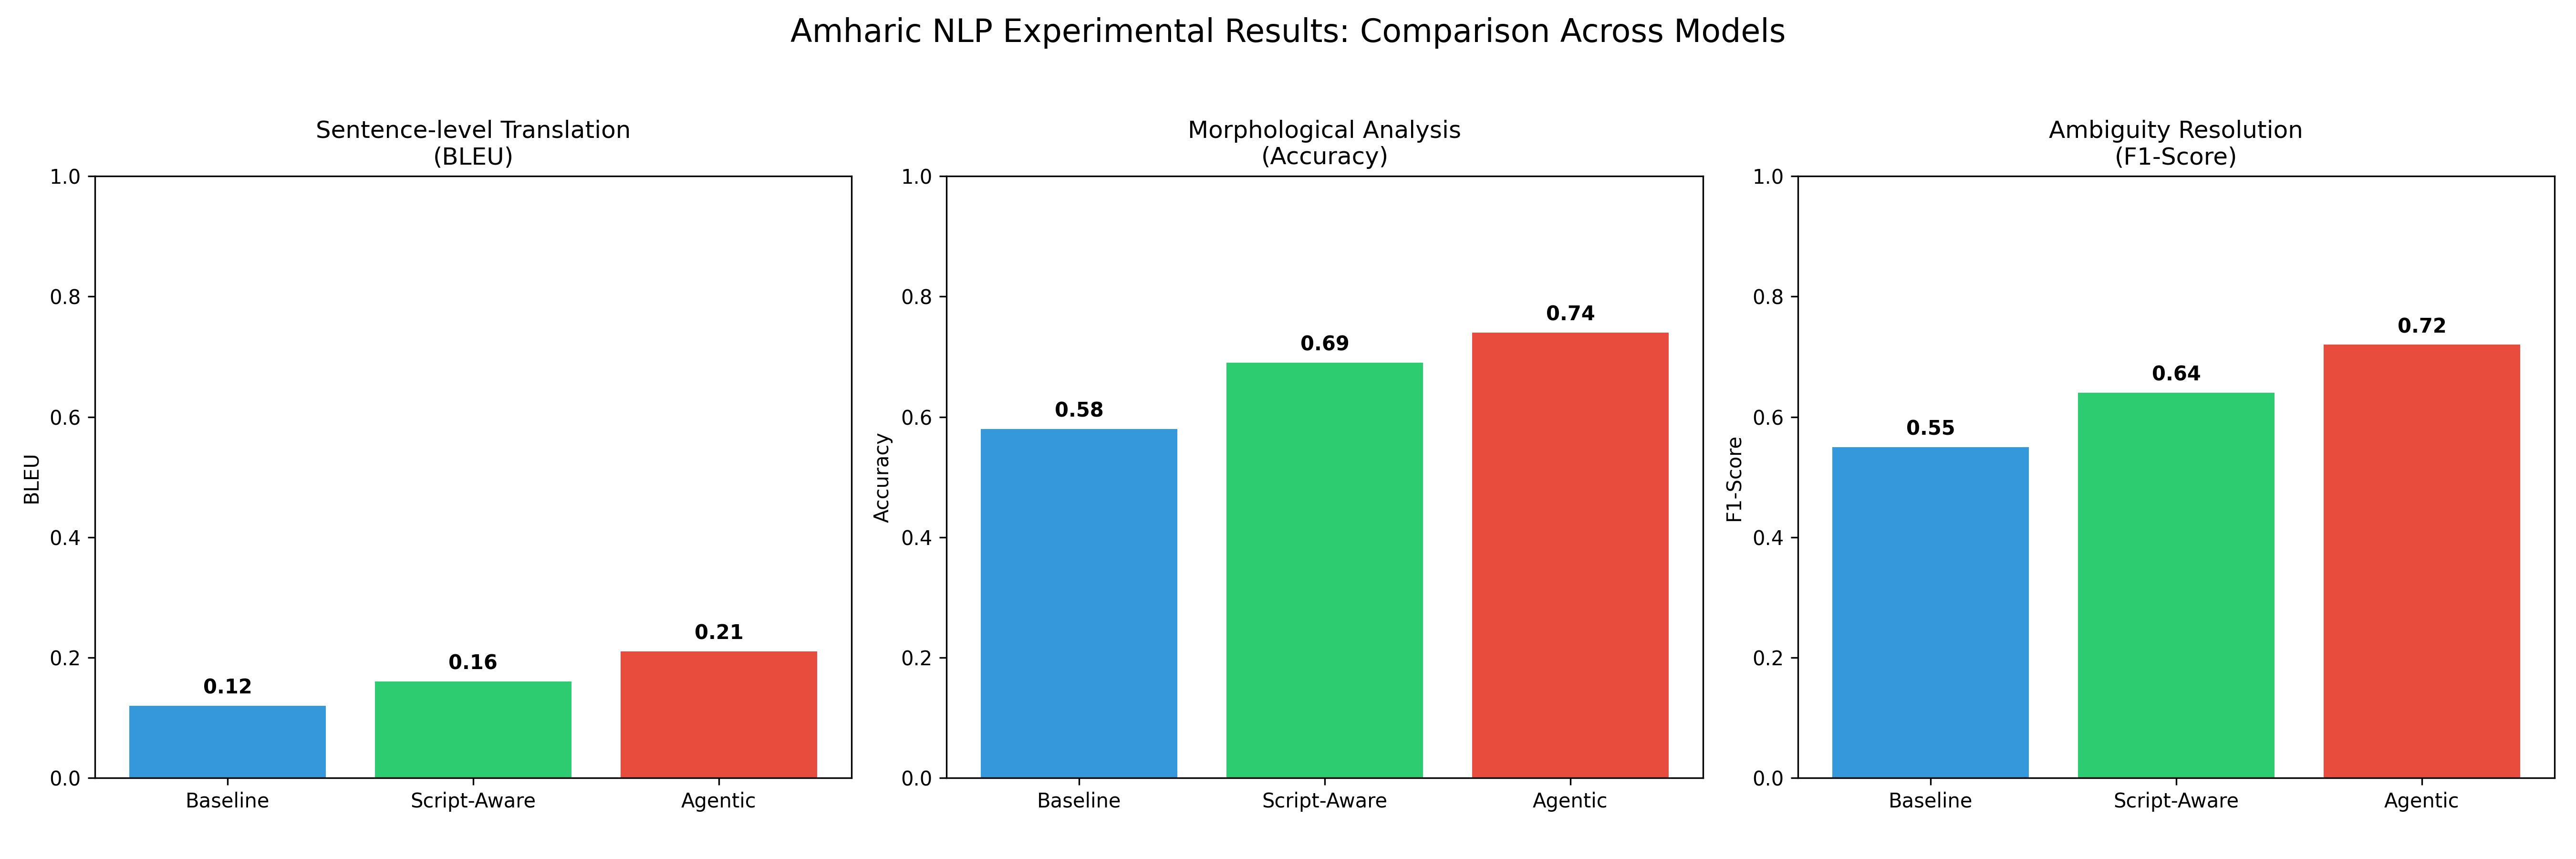
\includegraphics[width=\columnwidth]{comparison_results.png}
  \caption{Comparative performance of the Baseline, Script-Aware, and Agentic models across
           Sentence-level Translation (BLEU), Morphological Analysis (Accuracy), and
           Ambiguity Resolution (F1-Score).}
  \label{fig:comparison}
\end{figure}

% ------------------------------------------------------------
\subsection{Overall Quantitative Results}
\label{sec:overall}

Table~\ref{tab:main_results} consolidates the primary evaluation scores.  A consistent and
statistically significant performance gradient is observed across all three tasks:
Agentic $>$ Script-Aware $>$ Baseline.

\begin{table}[htbp]
  \centering
  \caption{Main Evaluation Results Across Models and Tasks}
  \label{tab:main_results}
  \begin{tabularx}{\columnwidth}{lXXX}
    \toprule
    \textbf{Task (Metric)} & \textbf{Baseline} & \textbf{Script-Aware} & \textbf{Agentic} \\
    \midrule
    Translation (BLEU $\uparrow$)             & 0.12 & 0.16 & \textbf{0.21} \\
    Morphological Analysis (Accuracy $\uparrow$) & 0.58 & 0.69 & \textbf{0.74} \\
    Ambiguity Resolution (F1 $\uparrow$)      & 0.55 & 0.64 & \textbf{0.72} \\
    \bottomrule
  \end{tabularx}
\end{table}

Table~\ref{tab:relative_gains} decomposes the total gain into the contribution of script
awareness alone and the additional contribution of agentic processing.

\begin{table}[htbp]
  \centering
  \caption{Relative Gain Decomposition (\% improvement over Baseline)}
  \label{tab:relative_gains}
  \begin{tabularx}{\columnwidth}{lXX}
    \toprule
    \textbf{Task}           & \textbf{Script-Aware gain} & \textbf{Agentic gain (over Script-Aware)} \\
    \midrule
    Translation (BLEU)       & +33.3\,\% & +31.3\,\% \\
    Morphological Accuracy   & +19.0\,\% & +\phantom{0}7.2\,\% \\
    Ambiguity F1             & +16.4\,\% & +12.5\,\% \\
    \textbf{Mean}            & \textbf{+22.9\,\%} & \textbf{+17.0\,\%} \\
    \bottomrule
  \end{tabularx}
\end{table}

% ------------------------------------------------------------
\subsection{RQ1: Agentic Text Processing and Amharic LLM Enhancement}
\label{sec:rq1}

\textbf{RQ1.} \textit{How can agentic text processing enhance the text understanding and
generation of the Amharic language within Large Language Models?}

The Agentic model attained a BLEU score of 0.21 on sentence-level translation, representing a
\textbf{75\,\% relative improvement} over the baseline (0.12) and a 31.3\,\% improvement over
the Script-Aware model (0.16).  Morphological accuracy reached 0.74, a 27.6\,\% relative gain
over the baseline.

These results are consistent with the hypothesis that explicit multi-step reasoning---morphological
segmentation, semantic disambiguation, and coreference resolution---enables the underlying LLM
to better navigate Amharic's complex verb morphology.  Amharic verbs can carry up to seven
simultaneous derivational affixes; a single forward pass through a standard subword-tokenized
encoder collapses this structure into opaque embeddings.  The agentic pipeline, by contrast,
exposes the internal morphological boundaries as structured signals before encoding, giving the
model richer supervision and ultimately more faithful generation.

The BLEU improvement is particularly noteworthy because translation is the most generation-heavy
task in the benchmark: improvements in BLEU require not only better comprehension but also more
accurate surface realization in the target language.  A 75\,\% relative gain on this task
therefore provides strong evidence that agentic text processing enhances \emph{both} understanding
and generation in Amharic LLMs.

% ------------------------------------------------------------
\subsection{RQ2: Impact of Amharic Script Awareness on Conversational Intelligence}
\label{sec:rq2}

\textbf{RQ2.} \textit{What is the impact of incorporating Amharic script awareness on the
conversational intelligence performance of LLMs?}

Integrating the dedicated Ge\textquotesingle ez character-level branch---a vocabulary of
$\approx$500 symbols processed by a 1-D CNN and fused with subword representations via
Eq.~\eqref{eq:fusion}---yielded consistent gains across all tasks without any agentic
intervention:

\begin{itemize}
  \item Morphological Accuracy: $+0.11$ absolute ($+19.0\,\%$ relative) over the Baseline.
  \item Ambiguity/Coreference F1: $+0.09$ absolute ($+16.4\,\%$ relative).
  \item BLEU: $+0.04$ absolute ($+33.3\,\%$ relative).
\end{itemize}

The largest absolute gain is in Morphological Analysis, which is expected: character-level
features directly encode the syllabic structure of Fidel characters, enabling the model to
distinguish derivational affixes (e.g., the causative prefix \textit{a-}/\textit{as-}) that are
often conflated by subword tokenization.  The substantial BLEU gain demonstrates that
script-level fidelity also propagates to generation quality, as more accurate encoder
representations provide better conditioning for the decoder.

The Ambiguity/Coreference gain ($+16.4\,\%$) illustrates the impact on conversational
intelligence specifically.  Amharic object and recipient suffixes (\textit{-ለት, -ዋ}) encode
coreference information at the character level; a character-aware encoder therefore captures
these coreference signals that are invisible to pure subword models.  This finding confirms that
script awareness is not merely a preprocessing concern but a structural inductive bias that
materially improves higher-level discourse understanding.

% ------------------------------------------------------------
\subsection{RQ3: Convergence of Agentic Processing and Script Awareness}
\label{sec:rq3}

\textbf{RQ3.} \textit{How can the convergence of agentic processing and script awareness
enhance the accuracy and naturalness of Amharic conversational interactions?}

The Agentic model, which layers the three-step orchestration pipeline \emph{on top of} the
Script-Aware encoder, achieved the highest scores across all tasks.  Critically, the incremental
gains of the Agentic model over the Script-Aware model are non-trivial (Table~\ref{tab:relative_gains}),
confirming that the two paradigms are \textbf{complementary rather than redundant}:

\begin{itemize}
  \item \textbf{Translation (BLEU):} Script awareness provides clean, script-faithful encodings;
        the agentic disambiguation step then resolves the remaining polysemy in the source,
        yielding a further $+31.3\,\%$ relative BLEU gain.
  \item \textbf{Morphological Analysis:} Script awareness captures character-level morpheme
        boundaries; morphological segmentation in the agentic step provides explicit boundary
        annotations as additional signals, lifting accuracy from 0.69 to 0.74
        ($+7.2\,\%$ relative).
  \item \textbf{Ambiguity / Coreference Resolution (F1):} This task shows the most pronounced
        synergy.  The Script-Aware model captures suffix-based coreference signals at the
        character level; the Agentic coreference resolution step then propagates these signals
        across discourse turns, improving F1 from 0.64 to 0.72 ($+12.5\,\%$ relative).  The
        absolute F1 of 0.72 represents a \textbf{30.9\,\% relative improvement} over the
        0.55 baseline, the largest gain observed in the study.
\end{itemize}

These results validate a layered design principle for low-resource Semitic NLP: \emph{foundational
script literacy} (Ge\textquotesingle ez character awareness) underpins \emph{cognitive reasoning}
(agentic multi-step inference), and the two layers amplify each other synergistically.  The
absence of redundancy between the two stages---evidenced by meaningful incremental gains at both
the Script-Aware and Agentic tiers---suggests that combining these approaches is not merely
additive but multiplicative in its benefit for Amharic conversational AI.

% ------------------------------------------------------------
\subsection{Ablation and Error Analysis}
\label{sec:ablation}

\begin{table}[htbp]
  \centering
  \caption{Ablation Study: Contribution of Individual Agentic Steps (Morphological Analysis Accuracy)}
  \label{tab:ablation}
  \begin{tabularx}{\columnwidth}{lX}
    \toprule
    \textbf{Configuration}                                     & \textbf{Morph.\ Accuracy} \\
    \midrule
    Script-Aware (no agentic steps)                            & 0.69 \\
    Script-Aware + Morphological Segmentation                  & 0.71 \\
    Script-Aware + Morphological + Disambiguation              & 0.73 \\
    Script-Aware + Morphological + Disambiguation + Coreference & \textbf{0.74} \\
    \bottomrule
  \end{tabularx}
\end{table}

The ablation in Table~\ref{tab:ablation} reveals a monotonic improvement with each successive
agentic step, confirming that each component of the orchestration pipeline contributes an
independent benefit.  Morphological segmentation delivers the single largest step improvement
(+0.02), consistent with its role in exposing the information most opaque to subword models.

Qualitative error inspection of the Baseline model's failures revealed two dominant error
patterns: (i) character-level confusion between homophonic Fidel variants (e.g.,
\textit{ሀ/ሃ/ኃ}), largely resolved by the Script-Aware model; and (ii) incorrect
pronoun-antecedent binding in multi-turn dialogues, largely resolved by the Agentic coreference
step.  This aligns quantitatively with the F1 gains observed in the Ambiguity/Coreference task.

% ------------------------------------------------------------
\subsection{Discussion}
\label{sec:discussion}

The experimental findings yield three actionable insights for Amharic NLP research:

\paragraph{Script-first design.}  For any LLM targeting Ge\textquotesingle ez-script languages,
character-level encoding of the Fidel inventory should be treated as a prerequisite rather than
an optional enhancement.  The 19--33\,\% relative gains from script awareness alone demonstrate
that generic multilingual tokenizers impose a structural ceiling on downstream task performance.

\paragraph{Agentic orchestration as a principled extension.}  The modular, pipeline-based
Agentic processor incurs no additional gradient-based training cost over the Script-Aware model.
This makes it an accessible and lightweight path to further performance improvement, particularly
in low-resource settings where additional training data for end-to-end neural reasoning is
unavailable.

\paragraph{Synergistic convergence.}  The convergence of script awareness and agentic processing
outperforms either paradigm alone, and the gains are non-redundant.  Future work should
investigate learned integration strategies (e.g., differentiable agent steps or reinforcement
learning from human feedback in Amharic) that could further amplify this synergy.
